\chapter{Prototypical Implementation of the Concept}
From the source scene point cloud, a prototype point cloud (person \acrshort{pcd}) is extracted. A region of interest (\acrshort{roi}) is defined in the source scene point cloud which contains the prototype point cloud. Geometric features are calculated for the selected region of interest. Non-prototype points are filtered out based on the geometric feature values of the points. Thus a prototype \acrshort{pcd} is obtained from the source scene \acrshort{pcd}. The acquired prototype point cloud is transformed into a target location on the target scene \acrshort{pcd}. The point cloud for the prototype is recalculated on the target scene \acrshort{pcd} based on the location of the prototype on the target scene \acrshort{pcd}. Surface reconstruction and Raycasting are used for the recalculation of points of the prototype point cloud. Thus obtained point cloud of the prototype after raycasting is termed as Raycasted Prototype \acrshort{pcd}. Shadow projected by the raycasted prototype point cloud on the target scene cloud is computed. Hence a new scenario of the target scene point cloud is created by the recombining of source scene \acrshort{pcd} and target scene \acrshort{pcd}. The following section explains each step in detail. For the purpose of the experiment, semantic-lidar data captured from \acrshort{carla} was used for both the source scene point cloud and target scene point cloud.

\section{Loading a Source Scene Point Cloud}
 In the figure \ref{fig:result-prototype_on_source_scene}, we can see points in the point cloud that are either black or green in color. To color the scene, we have used the ObjIdx value from the semantic-lidar data obtained from \acrshort{carla}. The semantic LIDAR data is sourced from CARLA to only facilitate the visualization of the prototype point cloud. The value of the ObjIdx is zero for stationery objects and the value of ObjIdx is non-zero for non-stationery objects. Based on this value, if the ObjIdx is 0 for point, the point is colored to green and if the ObjIdx is non-zero then the point is colored to black. In figure \ref{fig:result-prototype_on_source_scene}, we can see a prototype (person), located on the left part of the figure, represented by black in color. The point cloud in figure \ref{fig:result-prototype_on_source_scene} represents the \acrshort{carla} source scene as shown in functional implementation figure \ref{fig:functional_description_of_concept}.

\begin{figure}[htbp]
    \centering
    \begin{minipage}[b]{0.45\textwidth}
    \centering
    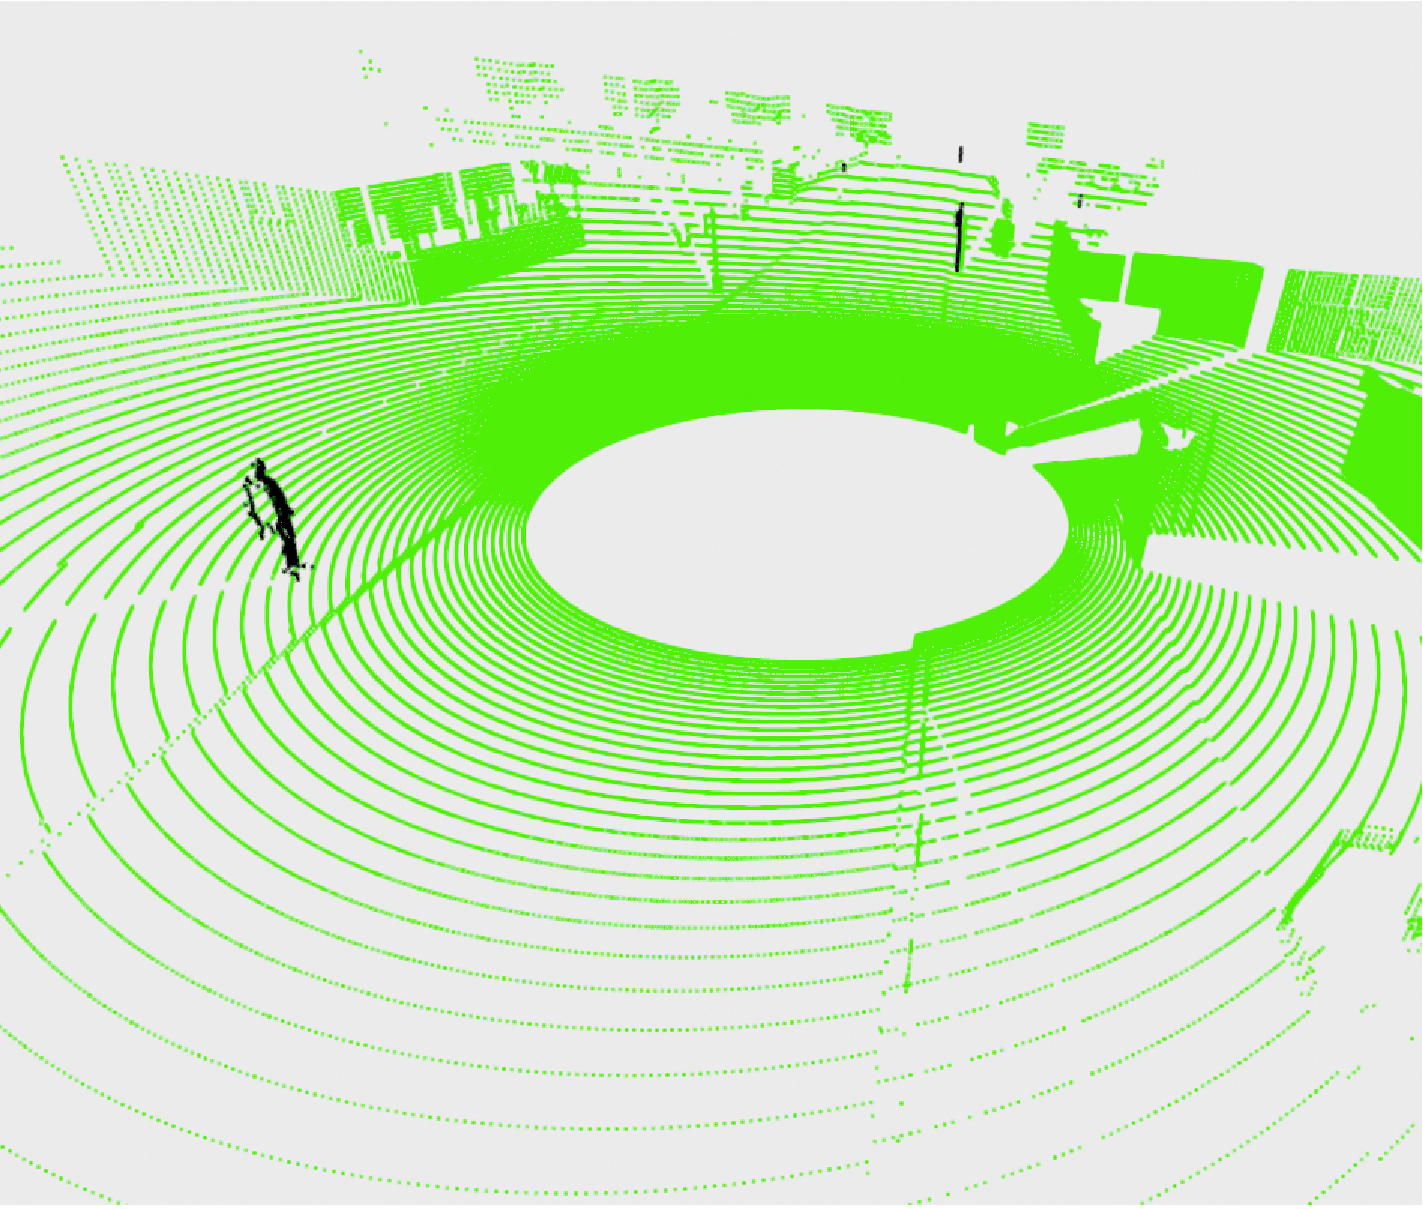
\includegraphics[width=1\linewidth]{97_graphics/results/prototype_on_source_scene_cloud.pdf}
    \caption{Prototype in Source Scene \acrshort{pcd}.}
    \label{fig:result-prototype_on_source_scene}
    \end{minipage}
    \hfill
    \begin{minipage}[b]{0.45\textwidth}
    \centering
    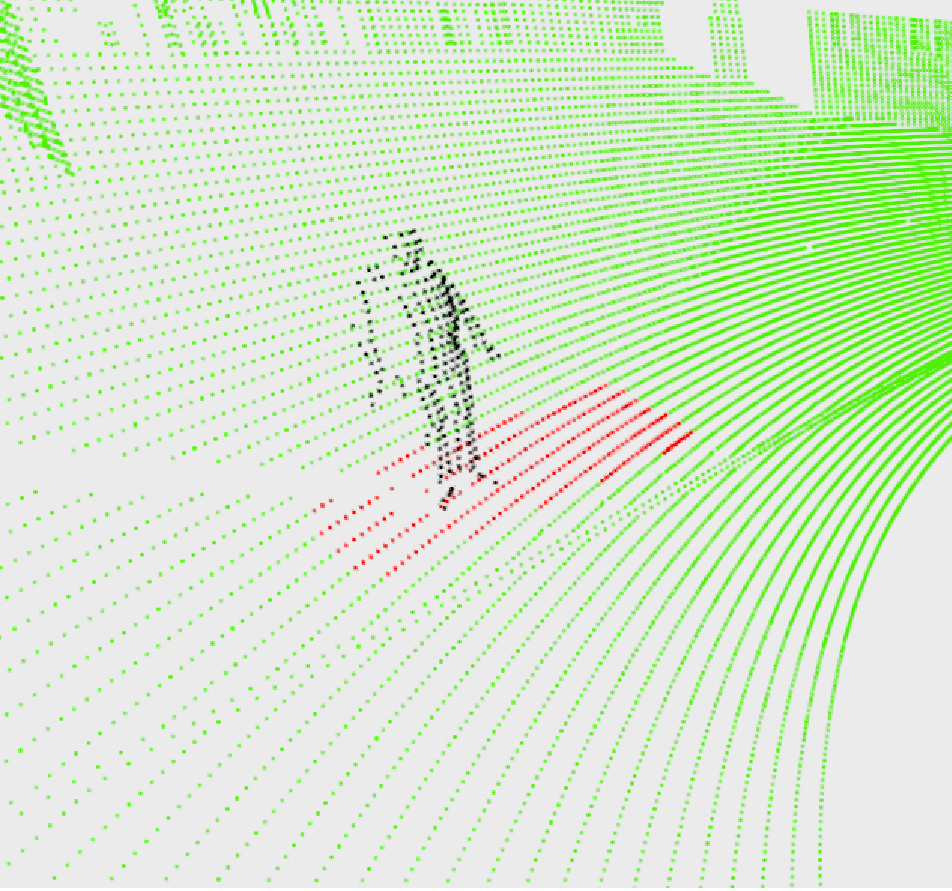
\includegraphics[width=1\linewidth]{97_graphics/results/roi_select_source_scene_cloud.pdf}
    \caption{Selection of \acrshort{roi} on Source Scene \acrshort{pcd}.}
    \label{fig:result-roi_select_source_scene}
    \end{minipage}
\end{figure}


\section{Selection of Region of Interest on Source Scene Point Cloud}
Since we plan on extracting the prototype from the source scene cloud, we need to specify the region on the source scene where we would like to extract the prototype \acrshort{pcd} from.

In figure \ref{fig:result-roi_select_source_scene}, the region of interest is represented by red-colored points plus any higher z-values points lying within the region. For ease of clarity, we have not changed the color of the prototype. First, a region is selected around the prototype manually. This is done manually by using the mouse cursor. At first, the position of the cursor is noted on the screen, if something is clicked on the screen then the relative position of the cursor on the world coordinates (the world where the point cloud is being visualized, the \acrshort{gui} for visualization) is calculated. Squared distances between the points on the point cloud and the world coordinate point are calculated. Based on minimum distance, a point on the point cloud is selected and marked with red color. Since manually selecting a list of points in a source scene cloud would take a lot of time, minimum x, minimum y, maximum x, and maximum y are calculated from the manually selected boundary region of interest. All the points that lie within the boundary value are finally selected as a region of interest on the source scene \acrshort{pcd}, from where a prototype \acrshort{pcd} is to be extracted.

\section{Extraction of Prototype from Source Scene Point Cloud}
Geometric features are calculated for the selected region of interest (\acrshort{roi}) from the source scene \acrshort{pcd}. Based on the number of nearest neighbors as 5 using "KDTreeSearchParamKNN" in open3d \parencite{open3d}, the nearest neighbor is searched for each point in the selected \acrshort{roi}. Using the kd-search tree, the covariance matrix and then the eigenvalue are computed after finding the local neighbors for each point in \acrshort{roi}. Utilizing the formulas for the calculation of geometric features as in equation \ref{eq:surf_var}, geometric features(surface variation) are calculated for each point in the \acrshort{roi} point cloud. The geometric feature values are filtered out by the appropriate threshold and finally, the remaining point having the valid geometric features in the selected \acrshort{roi} on the source scene \acrshort{pcd} is extracted, this extracted point cloud represents the prototype point cloud or original prototype point cloud.

\begin{figure}[htbp]
    \centering
    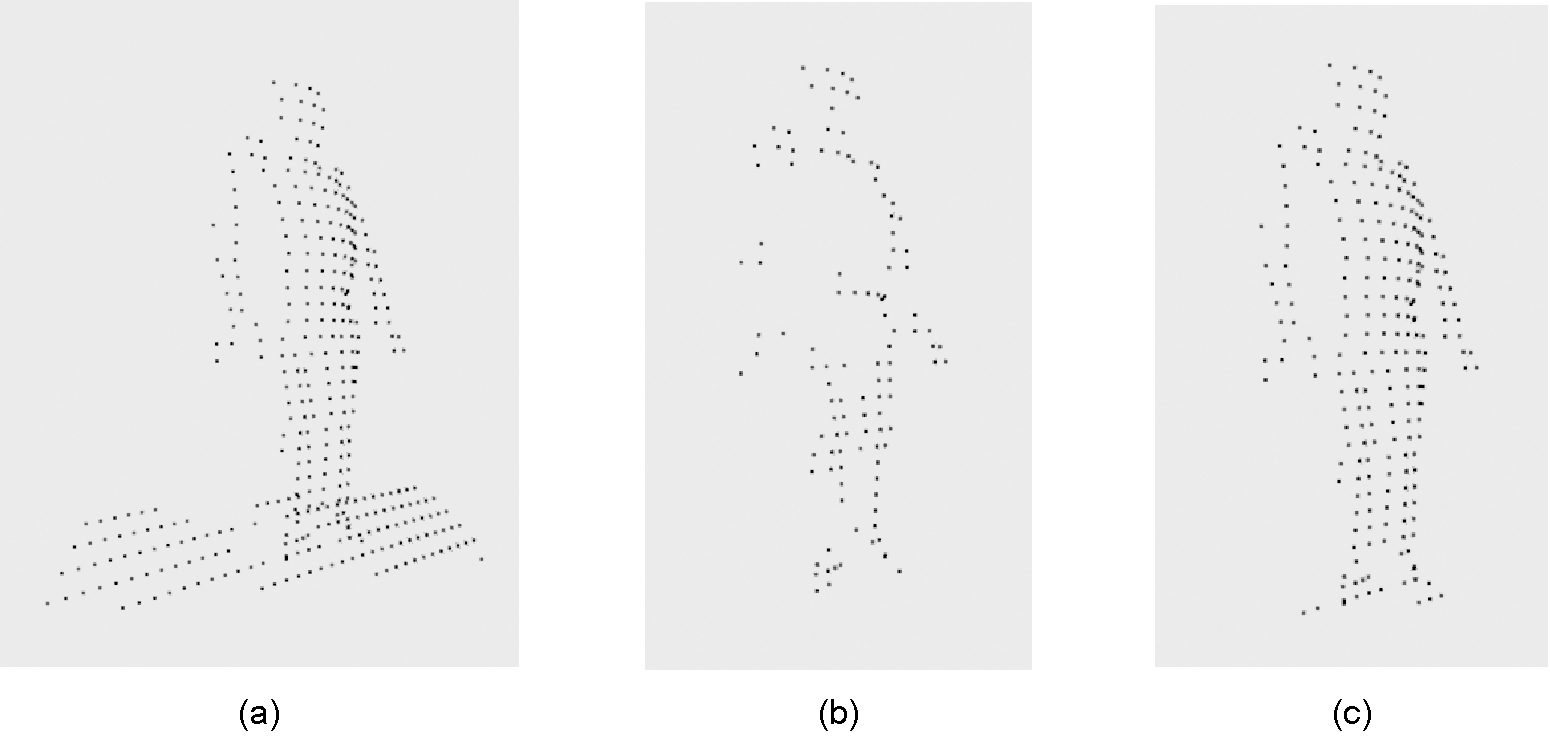
\includegraphics[width=0.8\linewidth]{97_graphics/results/prototype_extracted.pdf}
    \caption[Extracted Prototype Point Cloud from Source Scene \acrshort{pcd}.]{Extracted Prototype Point Cloud from Source Scene \acrshort{pcd} for different threshold of Surface Variation of points in selected \acrshort{roi} (a) \(Surface Variation \geq 0 \)  (b) \(Surface Variation \geq 0.05 \)  (c) \(Surface Variation \geq 10^{-8} \).}
    \label{fig:result-prototype_extracted}
\end{figure}

Trial and error were employed to explore different threshold values for surface variation, aiming to filter the prototype's point cloud optimally. As depicted in Figure \ref{fig:result-prototype_extracted}, a range of filtered point clouds for the prototype are displayed alongside their respective threshold values. Notably, the analysis reveals the utilization of a remarkably low threshold value \(10^{-8}\) for extracting the prototype's point cloud. This decision is attributed to the synthetic origin of the point cloud sourced from \acrshort{carla}, which lacks the randomness typically observed in the real-world LiDAR point clouds. The resulting point cloud obtained from this process is referred to as the "extracted prototype point cloud" or simply the "(original) prototype point cloud."

\section{Transformation of Prototype to a position on Target Scene Point Cloud}
The extracted prototype cloud could either be merged with the target scene \acrshort{pcd} on the original location (if the extracted prototype \acrshort{pcd} aligns properly with the target scene \acrshort{pcd}) or the prototype could also be transformed to a different location on the target scene \acrshort{pcd}.

\begin{figure}[htbp]
    \centering
    \begin{minipage}[b]{0.45\textwidth}
    \centering
    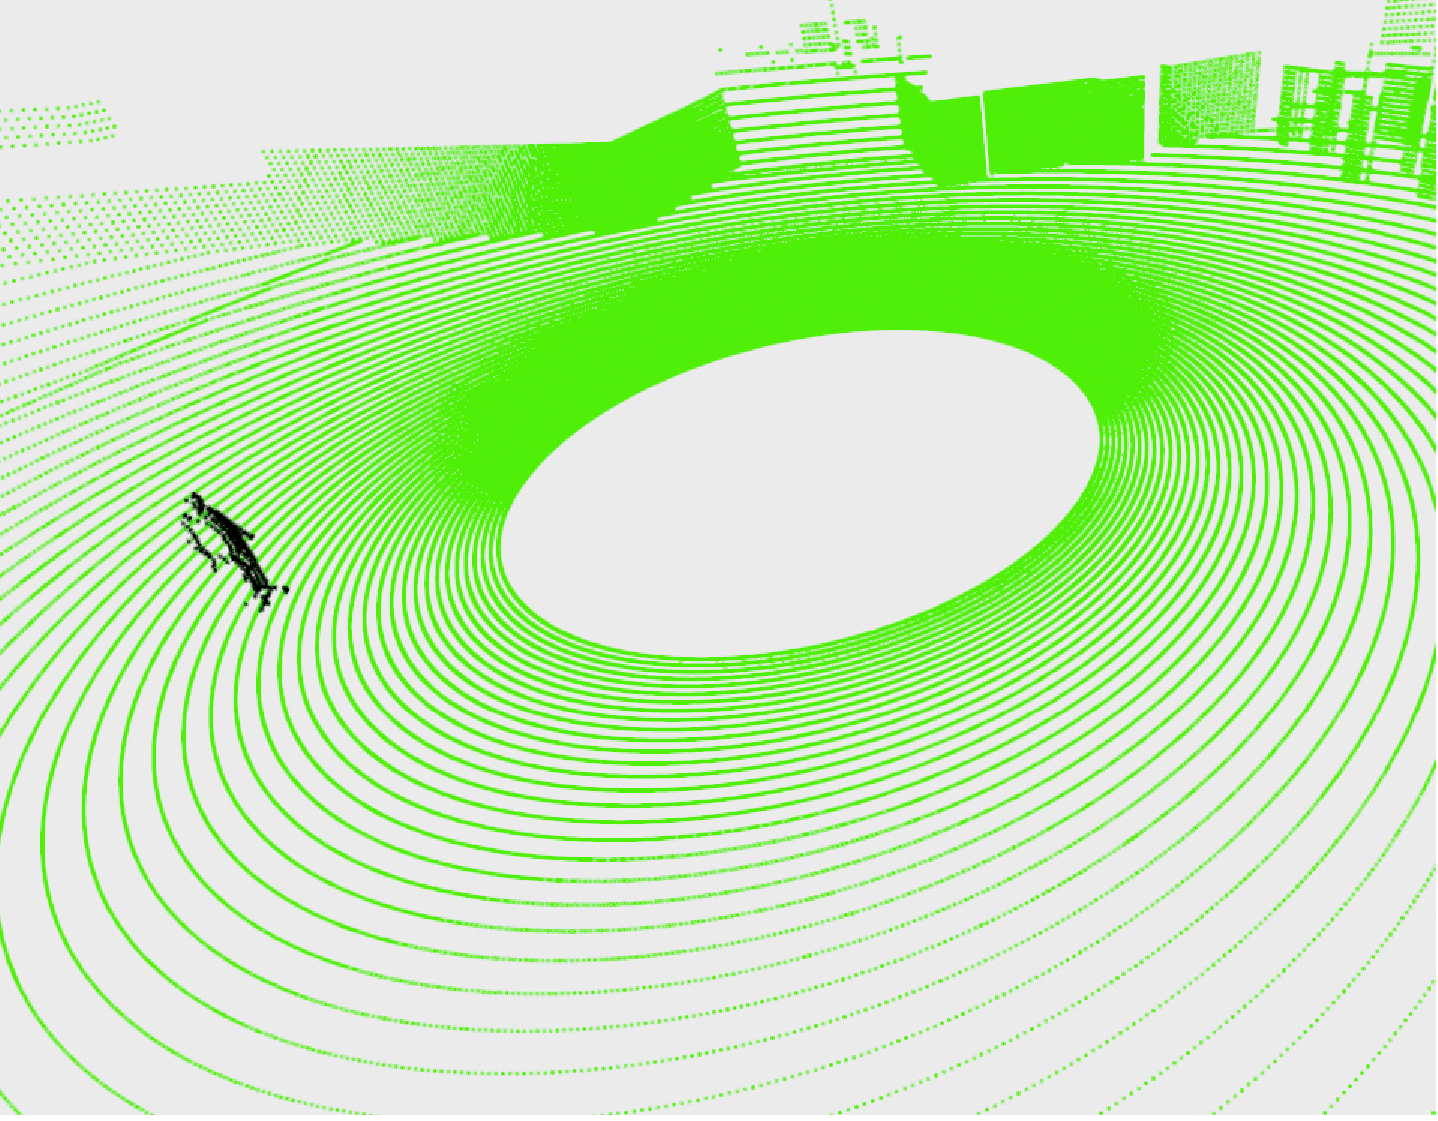
\includegraphics[width=1\linewidth]{97_graphics/results/prototype_on_target_scene_original_location.pdf}
    \caption{Prototype \acrshort{pcd} on Target Scene \acrshort{pcd} without transformation.}
    \label{fig:result-prototype_on_target_scene_original_location}
    \end{minipage}
    \hfill
    \begin{minipage}[b]{0.45\textwidth}
    \centering
    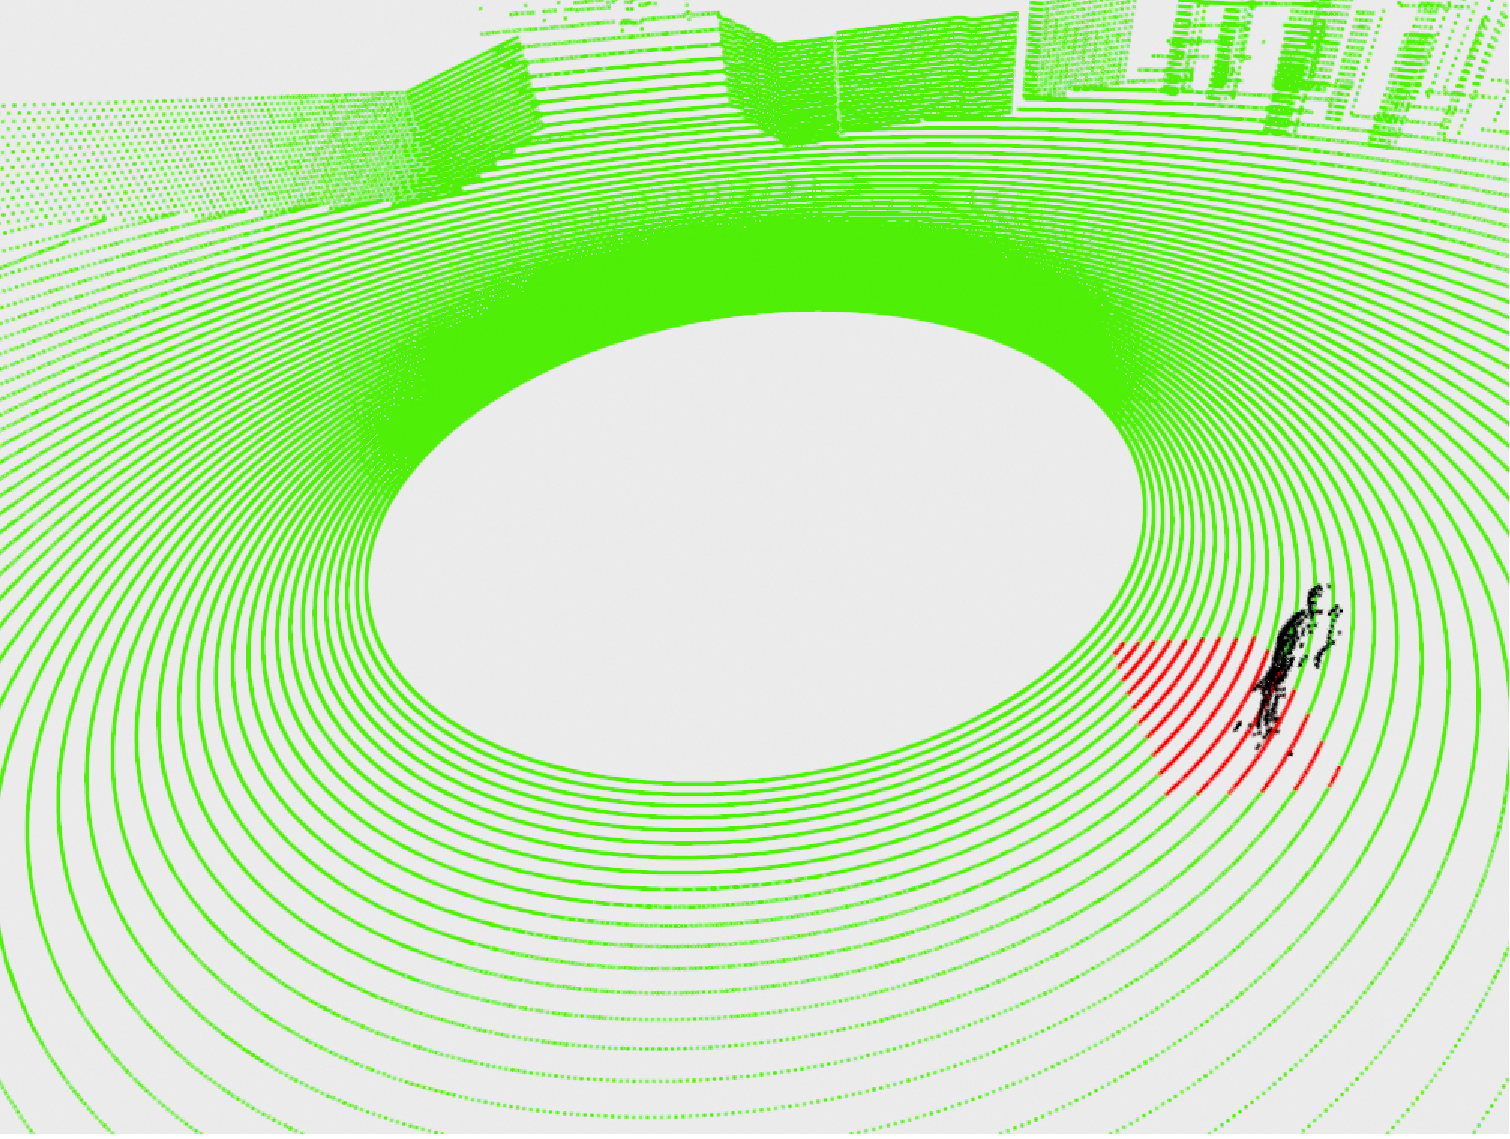
\includegraphics[width=1\linewidth]{97_graphics/results/prototype_on_target_scene_different_location.pdf}
    \caption{Prototype \acrshort{pcd} on Target Scene \acrshort{pcd} to a different position after transformation.}
    \label{fig:result-prototype_on_target_scene_different_location}
    \end{minipage}
\end{figure}

Figure \ref{fig:result-prototype_on_target_scene_original_location} shows a prototype \acrshort{pcd} (black points) without any transformation located on a target scene \acrshort{pcd}. Since the prototype is standing on top of the target scene and no irregularities were seen when concatenating the prototype point cloud (\acrshort{pcd})to the target scene point cloud (without transformation), we could also continue working with this position. Examples of irregularities encompass instances where a prototype appears submerged within the ground plane or traverses through a wall. If the prototype needs to be transformed to a different position, \acrfull{roi} is selected on the target scene point cloud. The selected ROI is shown by red colored points in figure \ref{fig:result-prototype_on_target_scene_different_location}. The translation and rotation matrix is calculated based on the reference centroid and target centroid as explained in figure \ref{fig:rotation_matrix_calculation}. One thing to note here is that when the position of the prototype is changed in figure \ref{fig:result-prototype_on_target_scene_different_location}, the prototype is also rotated according to the position change from the origin. Using the calculated rotational matrix, the prototype is rotated around the z-axis through the centroid of the prototype. This is an important step. Since we are not recalculating the side points or backside surfaces of a prototype, it is crucial to maintain the direction of the prototype relative to the origin. In our case, the prototype is still facing the origin.

\section{Surface Reconstruction and Filtering}
After the position of the prototype \acrshort{pcd} has been finalized on the target scene \acrshort{pcd}, the next step is the reconstruction of the surface. Using the Poisson reconstruction method, the surface of the prototype is reconstructed.

\begin{figure}[htbp]
    \centering
    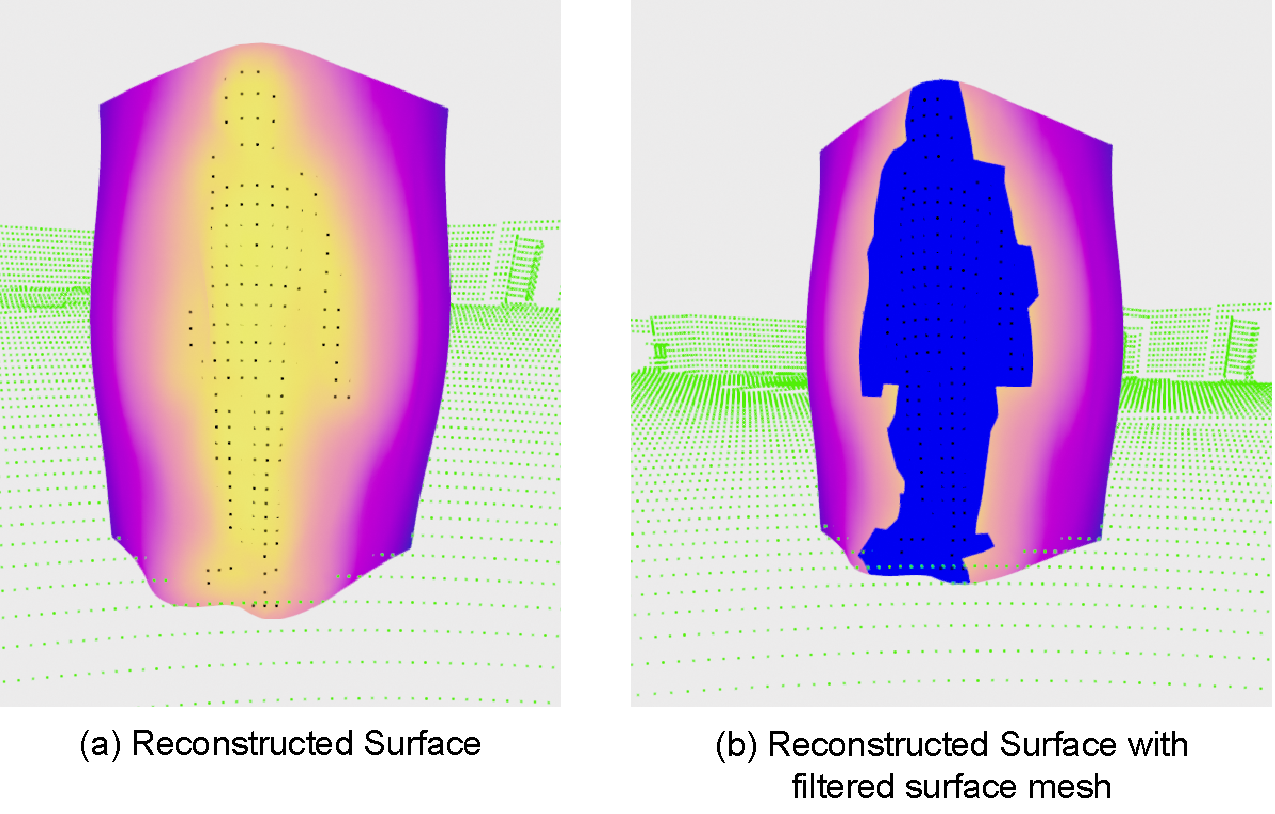
\includegraphics[width=1\linewidth]{97_graphics/results/surface_reconstruction.pdf}
    \caption[Reconstructed Surface of the Prototype on the Target Scene \acrshort{pcd}.]{Reconstructed Surface of the Prototype on the Target Scene \acrshort{pcd} (a) Reconstructed Surface with varying density of points (b) Reconstructed surface with filtered surface mesh (blue).}
    \label{fig:result-surface_reconstruction}
\end{figure}

Figure \ref{fig:result-surface_reconstruction} \((a)\) represents the total reconstructed surface visualized by varying density of points on the surface. The yellow color surface represents the region with a higher point density. The purple-colored surface in the figure represents the region with lower point density. The reconstructed surface of the prototype represents a triangle mesh. Since the prototype is relatively smaller than the reconstructed surface as shown in figure \ref{fig:result-surface_reconstruction} \((a)\), we need to filter the undesired surface of the reconstructed prototype. Using density value for filtering also works but requires lots of trial and error to get an optimal value, so we filtered the undesired reconstructed surface by removing all the triangle mesh that does not contain the point cloud of the prototype. This filtered surface of the prototype is represented by the blue color region in the figure \ref{fig:result-surface_reconstruction} \((b)\). It can be viewed that the filtered surface (represented by the blue color) tries to resemble the shape of the prototype with a higher concentration of point cloud. The depth information of the prototype points is represented by the varying depth of the triangles in the filtered reconstructed surface (triangle mesh).

\section{Raycasting}
Rays originating from the origin of the target scene \acrshort{pcd} and directed toward the point clouds in the region of interest are "created". The region of interest on the target scene \acrshort{pcd} is selected in such a way that the rays cover the surface of the filtered surface mesh as much as possible. The selected region on the target scene is represented by red color points.

\begin{figure}[htbp]
    \centering
    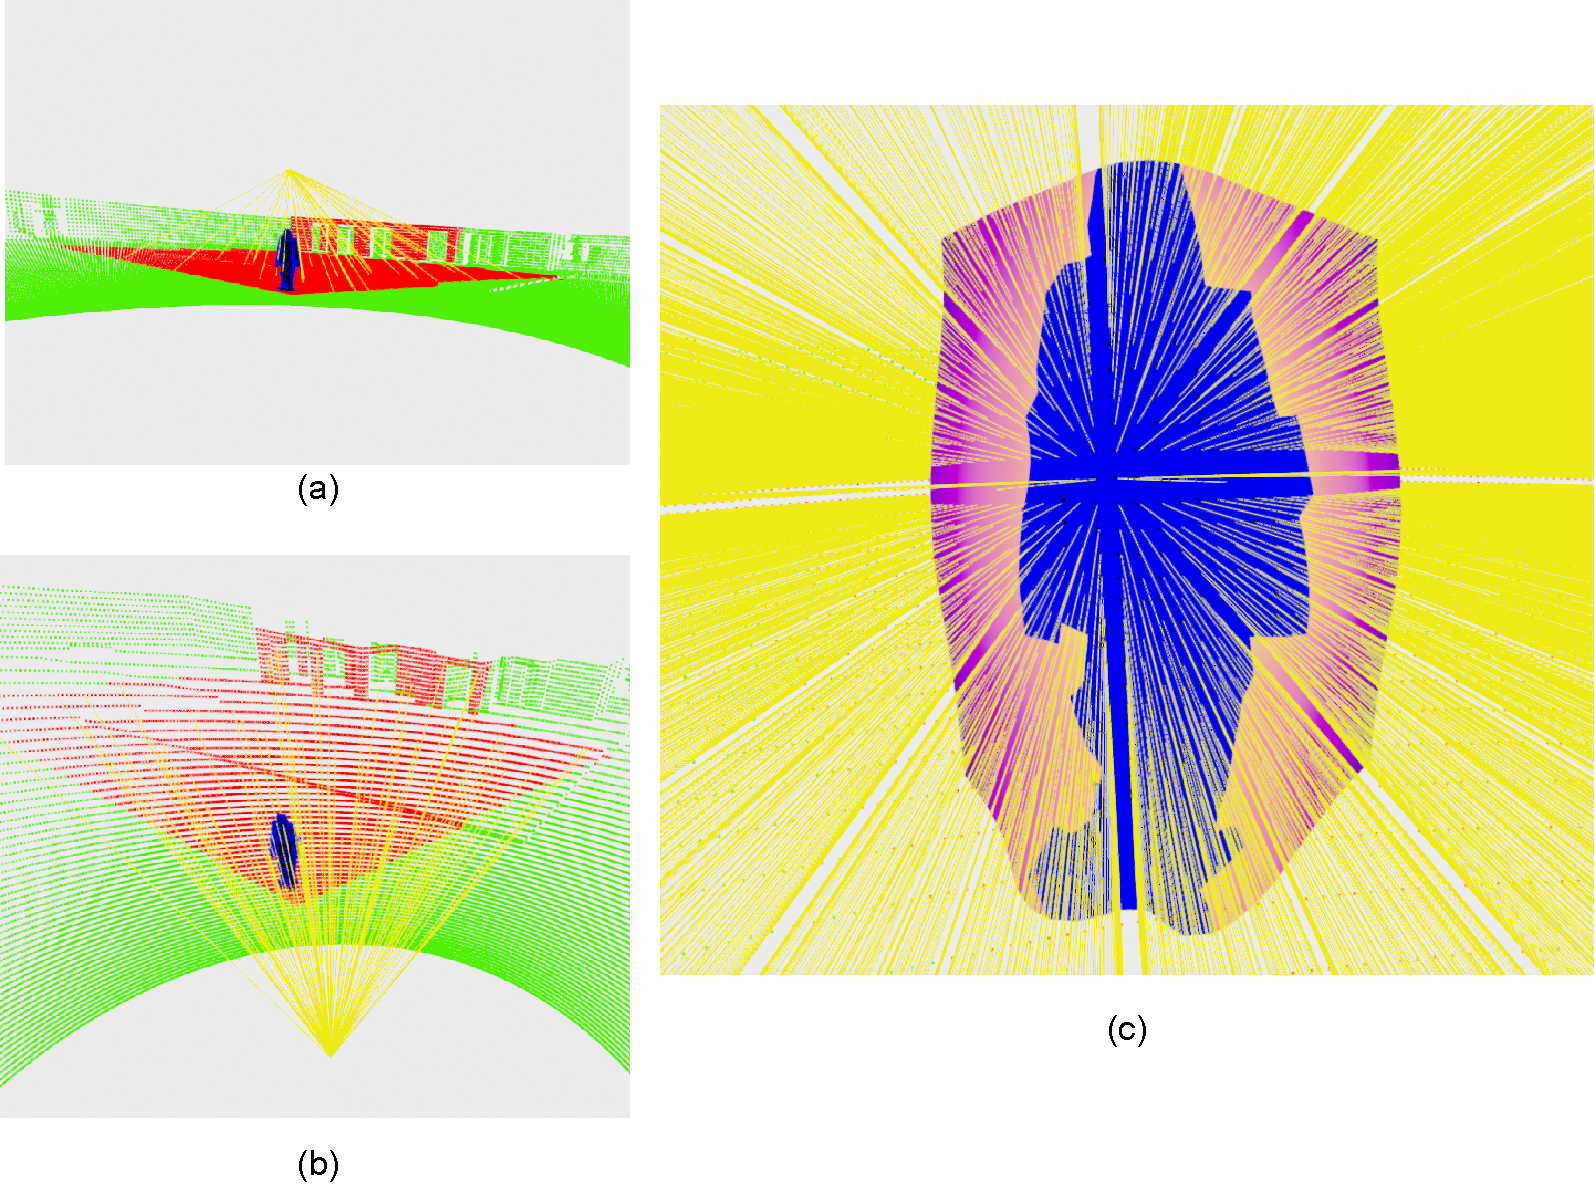
\includegraphics[width=1\linewidth]{97_graphics/results/raycasting_from_origin.pdf}
    \caption[Raycasting from Origin to the target \acrshort{roi} on the Target Scene Point Cloud (\acrshort{pcd}).]{Raycasting from Origin to the target \acrshort{roi} on the Target Scene Point Cloud (\acrshort{pcd}). (a) and (b) shows raycasting with a lower ray count. (c) shows rays intersect with the surface of the Prototype.}
    \label{fig:result-raycasting_from_origin}
\end{figure}

In the figure \ref{fig:result-raycasting_from_origin}, the yellow color lines mimic the laser rays from the LiDAR sensor. The blue color represents the surface mesh of the prototype after filtering. When the ray traverses from the origin to the target region of interest (\acrshort{roi}), it intersects the surface mesh. An example illustrating the triangle mesh and rays traversal is shown in figure \ref{fig:result-raycasting_with_triangles}.

\begin{figure}[htbp]
    \centering
    \begin{minipage}[b]{0.8\textwidth}
    \centering
    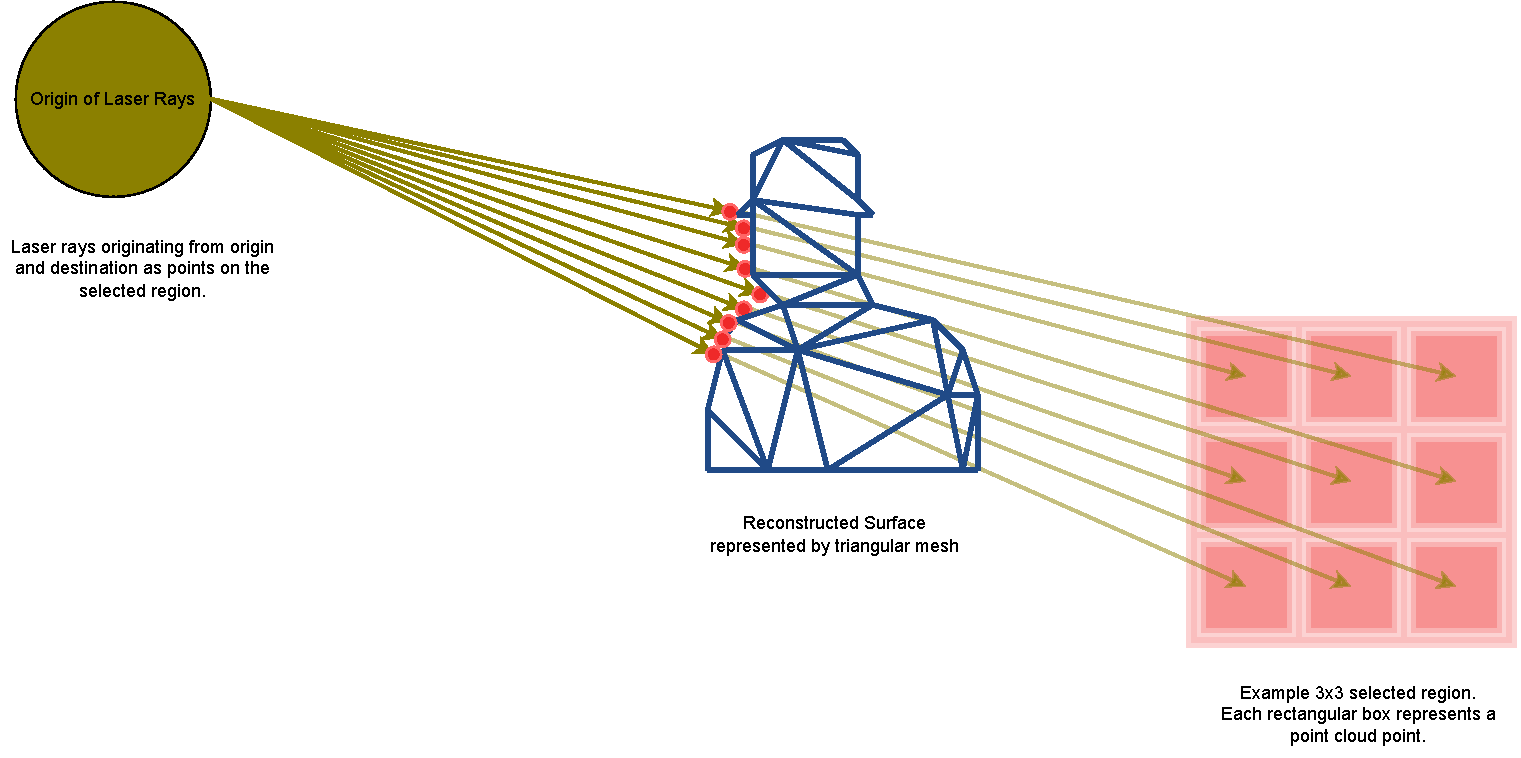
\includegraphics[width=1\linewidth]{97_graphics/results/raycasting_with_trianglesmeshes.pdf}
    \caption{Rays casting towards Prototype surface represented by a group of triangles in the triangle mesh.}
    \label{fig:result-raycasting_with_triangles}
    \end{minipage}
\end{figure}

Figure \ref{fig:result-raycasting_with_triangles} gives an example of a prototype surface represented by a group of triangles of a triangle mesh. Triangle intersected by the rays are calculated by casting rays as shown in figure \ref{fig:result-raycasting_from_origin}  and figure  \ref{fig:result-raycasting_with_triangles}. From the intersected triangles, new points of the prototype are calculated. 

\begin{figure}[htbp]
    \centering
    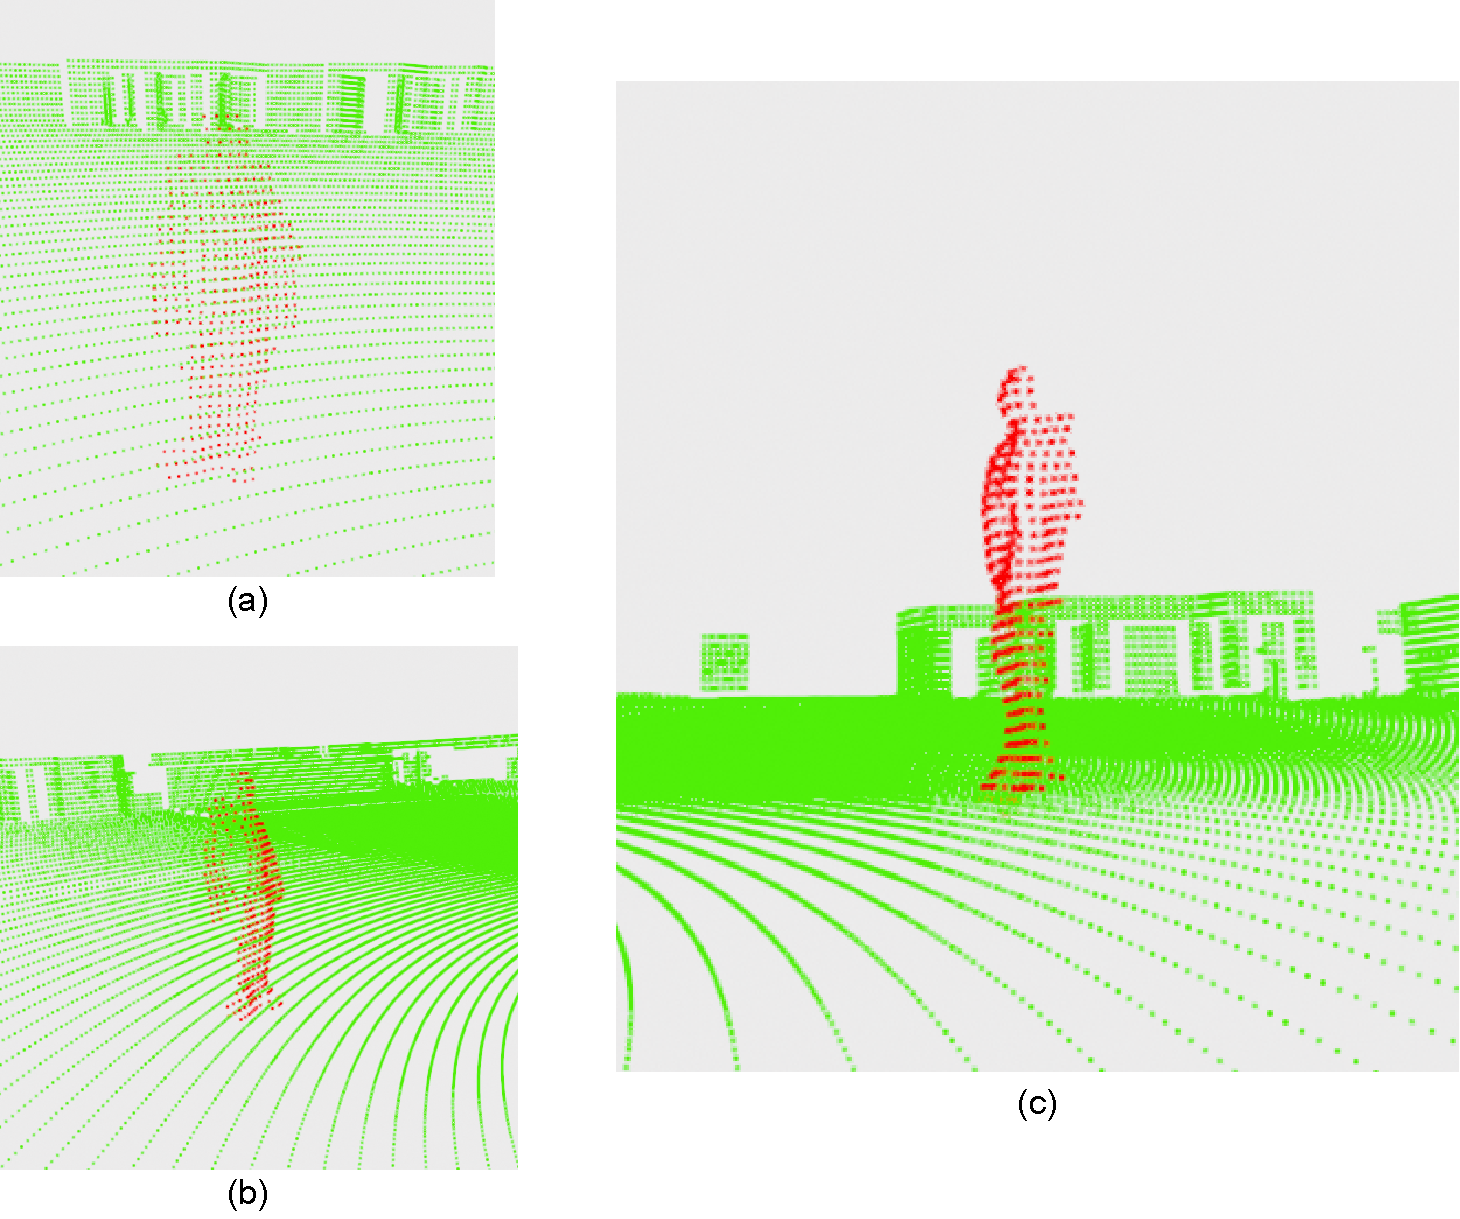
\includegraphics[width=0.6\linewidth]{97_graphics/results/raycasted_prototype.pdf}
    \caption{Raycasted Prototype visualized by red colored point cloud on the target scene cloud from different viewpoints.}
    \label{fig:result-raycasted_prototype}
\end{figure}

The raycasted point cloud of the prototype is calculated by using the equation \ref{eq:find_xyz} as shown in figure \ref{fig:concept-raycasting_single_triangle_by_t_hit}. As a final result, a point cloud of the prototype is created. We call the point cloud received after raycasting a raycasted prototype point cloud. Figure \ref{fig:result-raycasted_prototype} shows the raycasted point cloud of the prototype calculated after the raycasting method.
The red points point cloud represents the raycasted prototype in figure \ref{fig:result-raycasted_prototype}. It can be observed that the calculated point cloud of the surface mimics the surface of the original prototype (person). The raycasted prototype lies on the target scene \acrshort{pcd}. Shadow projection by the raycasted prototype on the target scene \acrshort{pcd} needs to be calculated. This is done in the next section.

\section{Shadow Casting on Target Scene by Raycasted Prototype Point Cloud}
The input to this step is a raycasted prototype point cloud on a target location (\acrshort{roi}) of the target scene \acrshort{pcd}. An experiment was done with the hidden point removal algorithm. Important parameters for the HPR algorithm are the viewpoint and the radius of the sphere for spherical flipping. Visibility of the points is determined by looking from the viewpoint of the target scene cloud. The viewpoint is set to the origin so that the process mimics the shadow projection process when a LiDAR sensor is placed at the origin. Appropriate parameters for the HPR algorithm need to be chosen to increase the shadow projection accuracy. As shown in figure \ref{fig:concept-shadow_casting_difference}, instead of using the HPR algorithm, the raycasted method is a more accurate approach for shadowcasting in our experiment. 

\begin{figure}[htbp]
    \centering
    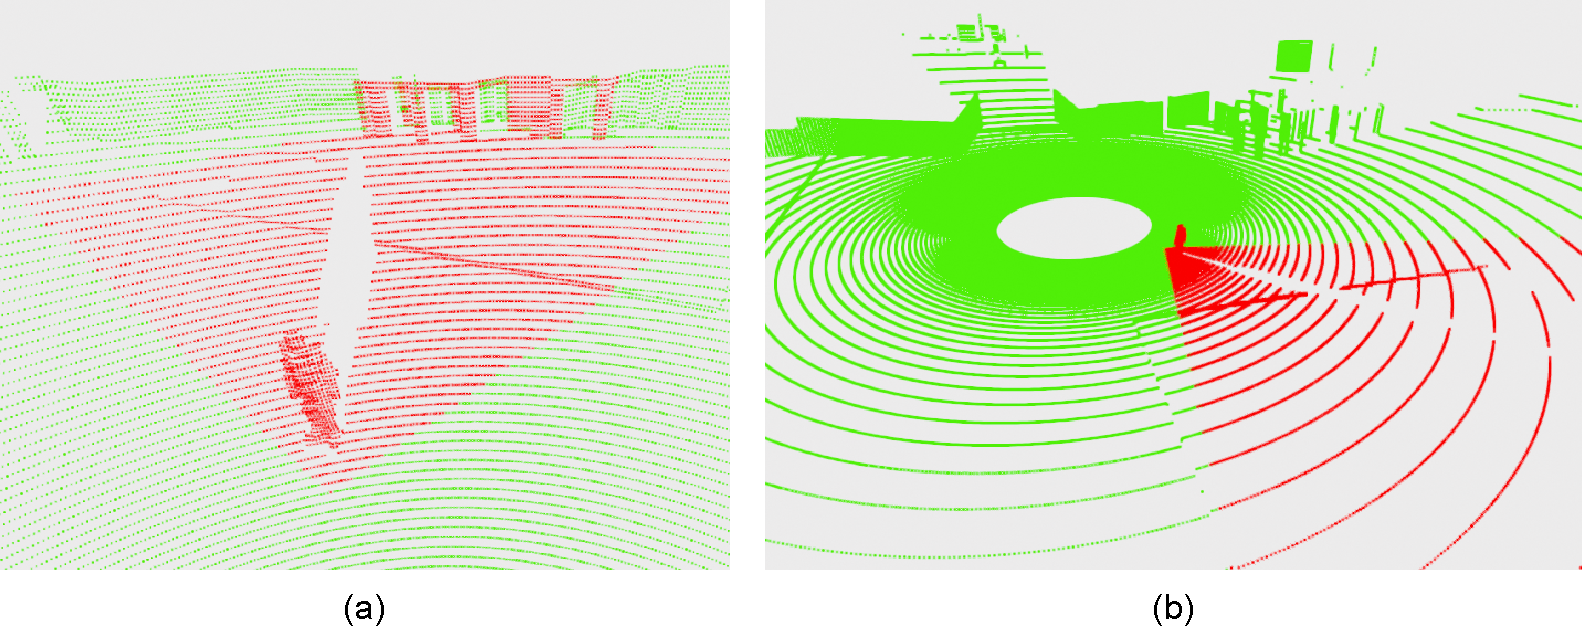
\includegraphics[width=1\linewidth]{97_graphics/results/shadow_casting_by_prototype.pdf}
    \caption{Shadow Casting by the Prototype on the Target Scene \acrfull{pcd}. (a) and (b) shows projected shadow from different viewpoints.}
    \label{fig:result-shadow_casting_by_prototype}
\end{figure}

Using the raycasted method as explained in figure \ref{fig:concept-shadow_casting_by_raycast_method}, the shadow projected by the prototype surface in the target region of the target scene cloud is calculated. The result of shadow casting is shown in figure \ref{fig:result-shadow_casting_by_prototype}. Points lying on the shadow region of the prototype are removed. Shadow was calculated for \acrshort{roi} to make the computation faster (shown by red colored region in figure \ref{fig:result-shadow_casting_by_prototype}).